
\textbf{Magic3D}~--~This method employs a coarse-to-fine methodology, aiming to first construct a basic outline of the target object, which is then refined in subsequent stages to more accurately align with the text prompt. The mesh initialization is random, mirroring the approach used in DreamFusion.

\begin{figure}[H]
    \centering
    % Subfigure for textual description
    \begin{subfigure}[b]{0.15\textwidth}
        \centering
        \fontsize{9pt}{7pt}\selectfont\text{Iteration 200}\vspace{3cm}
        \fontsize{9pt}{7pt}\selectfont\text{It. 5000}\vspace{2.85cm}
        \fontsize{9pt}{7pt}\selectfont\text{It. 10000}\vspace{1.95cm}
    \end{subfigure}
    \begin{subfigure}[b]{0.2\textwidth}
        \centering
        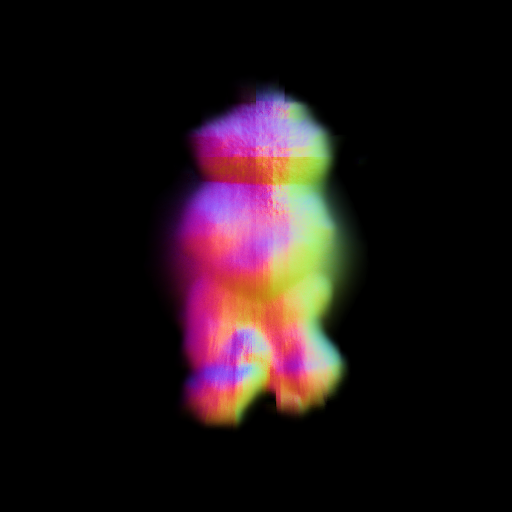
\includegraphics[width=\textwidth]{etc/a robot made out of plants/magic3d/magic3D_coarse_robot_0_part2.png}
        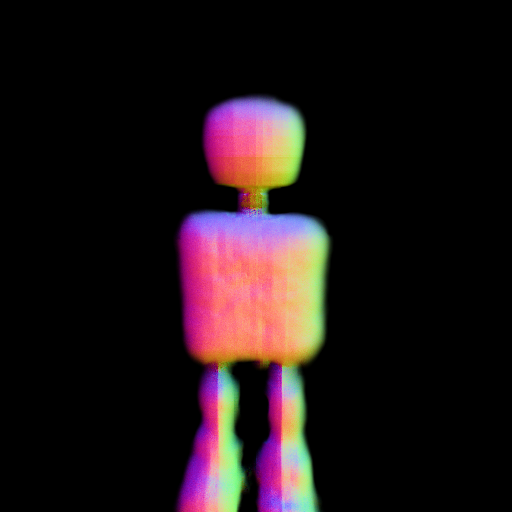
\includegraphics[width=\textwidth]{etc/a robot made out of plants/magic3d/magic3D_coarse_robot_5000_part2.png}
        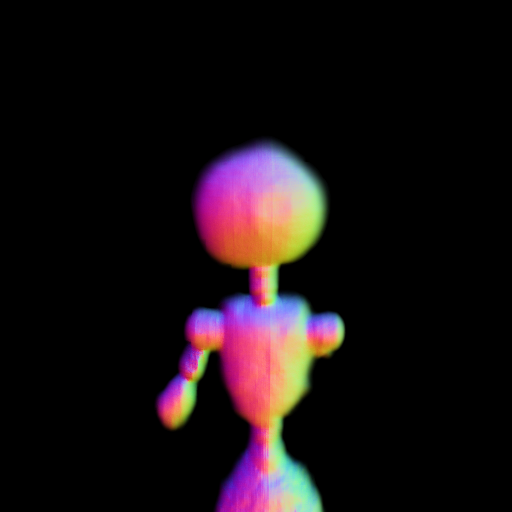
\includegraphics[width=\textwidth]{etc/a robot made out of plants/magic3d/magic3D_coarse_robot_10000_part2.png}
        \caption{}
    \end{subfigure}
    \begin{subfigure}[b]{0.2\textwidth}
        \centering
        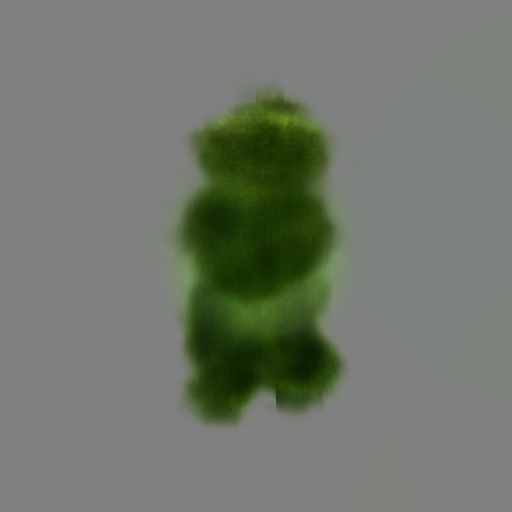
\includegraphics[width=\textwidth]{etc/a robot made out of plants/magic3d/magic3D_coarse_robot_0_part1.png}
        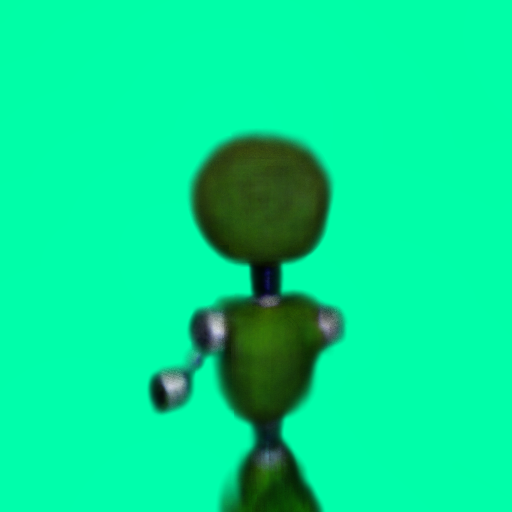
\includegraphics[width=\textwidth]{etc/a robot made out of plants/magic3d/magic3D_coarse_robot_5000_part1.png}
        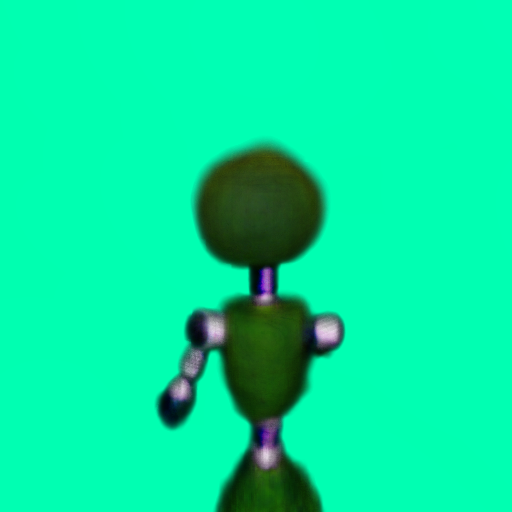
\includegraphics[width=\textwidth]{etc/a robot made out of plants/magic3d/magic3D_coarse_robot_10000_part1.png}
        \caption{}
    \end{subfigure}
    \begin{subfigure}[b]{0.2\textwidth}
        \centering
        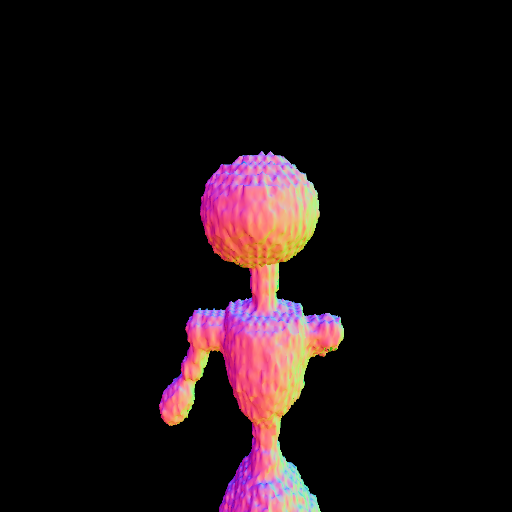
\includegraphics[width=\textwidth]{etc/a robot made out of plants/magic3d/magic3D_refine_robot_0_part2.png}
        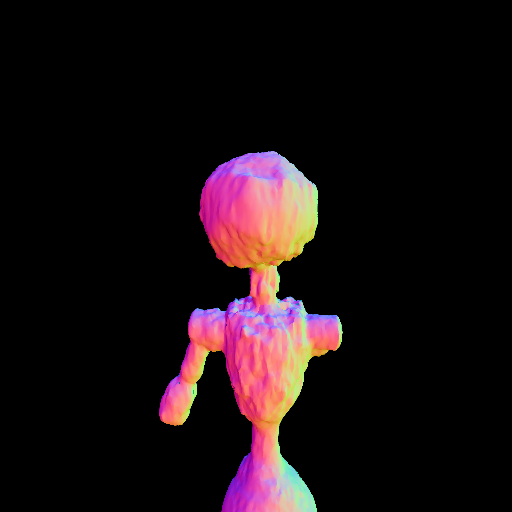
\includegraphics[width=\textwidth]{etc/a robot made out of plants/magic3d/magic3D_refine_robot_5000_part2.png}
        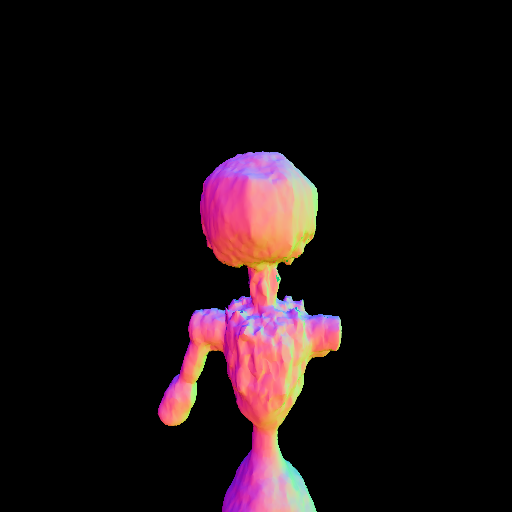
\includegraphics[width=\textwidth]{etc/a robot made out of plants/magic3d/magic3D_refine_robot_10000_part2.png}
        \caption{}
    \end{subfigure}
    \begin{subfigure}[b]{0.2\textwidth}
        \centering
        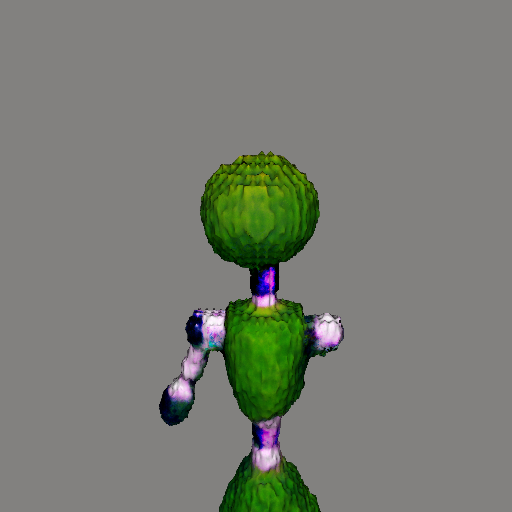
\includegraphics[width=\textwidth]{etc/a robot made out of plants/magic3d/magic3D_refine_robot_0_part1.png}
        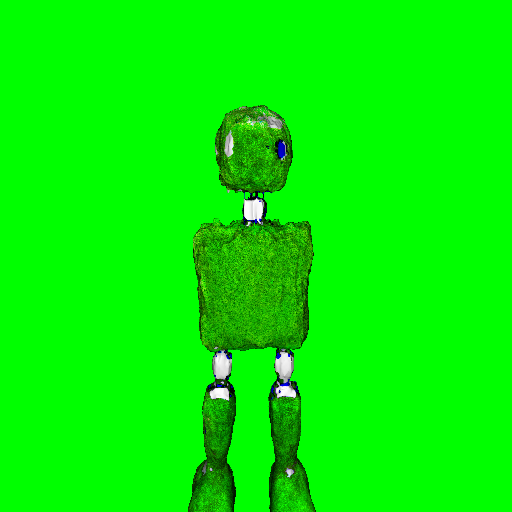
\includegraphics[width=\textwidth]{etc/a robot made out of plants/magic3d/magic3D_refine_robot_5000_part1.png}
        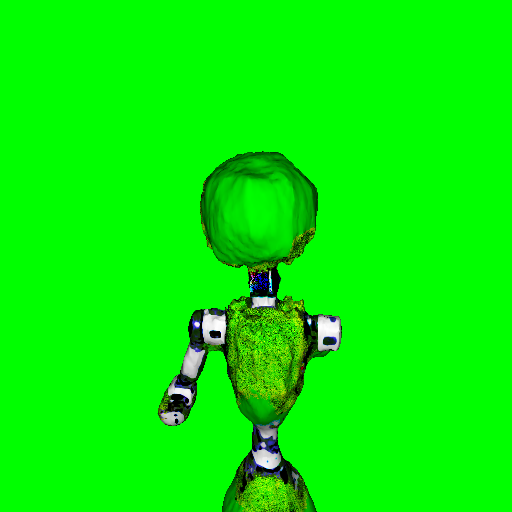
\includegraphics[width=\textwidth]{etc/a robot made out of plants/magic3d/magic3D_refine_robot_10000_part1.png}
        \caption{}
    \end{subfigure}
    \caption{Magic3D's generation process: Progress of the coarse stage in (a, b) and the refine stage in (c, d)}~\label{fig:generationMagic3D}
\end{figure} 

The coarse stage can be seen in Figure~\ref{fig:generationMagic3D} parts (a) and (b). From a random start, a rough shape starts emerging by Iteration 200, accompanied by a plant-like green hue, setting the foundation for further refinement. By Iteration 5000, significant transformations have occurred from the initial stage: a distinct circular head, a neck, the upper body of the robot, and one arm have formed. The lower body, however, was omitted during training, forcing subsequent refinements on the upper half. At this point, the arm's color diverges from the green base, taking on a rough, grey-metallic appearance. Progressing to Iteration 10000, the neck and certain parts of the hip also adopt this metallic color. Despite these changes, the overall shape of the model undergoes only minor adjustments between Iteration 5000 and 10000, such as a thicker left arm and a more pronounced hip, but the right arm remains entirely absent. From the coarse stage alone, the model vaguely indicates a robotic form, with the plant aspect being derived primarily from the green coloring.

In the refinement stage, parts (c) and (d), the process starts from the model generated in the coarse stage. Initially, the mesh appears blocky but retains its original shape, with the neck, shoulder, and hip areas acquiring a purple hue between Iterations 0 and 200. By Iteration 5000, the model is smoother, with minor modifications to the head, losing some of its roundness. However, not much else changes in shape. The texture, though, sees significant refinement; the arms, hip, and neck gain more detail, resembling parts of an actual robot. The chest acquires grass-like detail and coloration. By Iteration 10000, some of these textural details diminish, as evidenced by the stomach area reverting to a plain green. However, the model gains light reflections, particularly noticeable on the shoulders. Despite these changes, the model's shape remains largely unchanged from Iteration 5000 to 10000, and the missing arm issue persists through the refinement stage.

The final mesh, as displayed in Figure~\ref{fig:texturesMagic3D}, is recognizable as a robot, and with close inspection, one might discern its grass-like chest, suggesting a plant-themed robot. For immediate and clear identification, the model would benefit from enhanced detail, particularly a more developed lower body extending beyond the hips. The left side of the figure displays the albedo generated during training.

\begin{figure}[H]
    \centering
      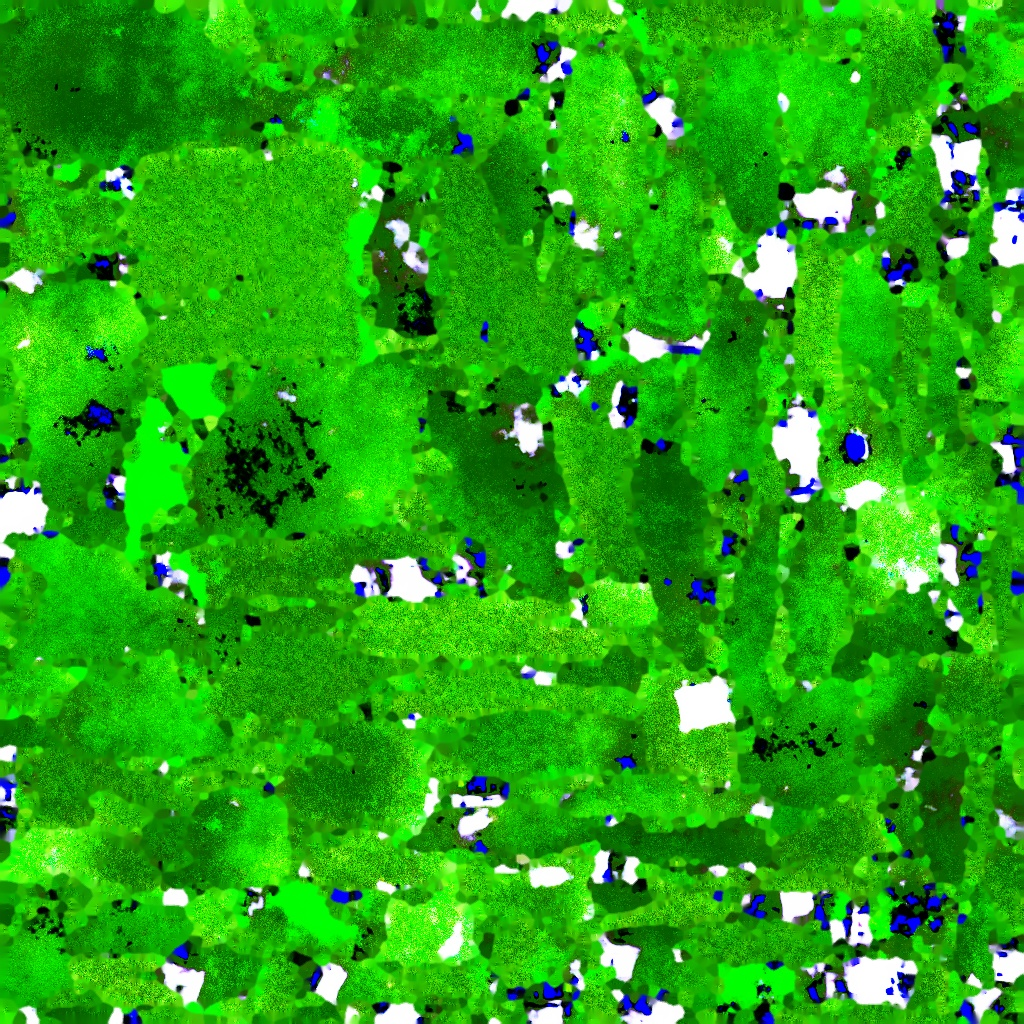
\includegraphics[width=.25\columnwidth]{etc/a robot made out of plants/magic3D/magic3D_refine_robot_texture}
      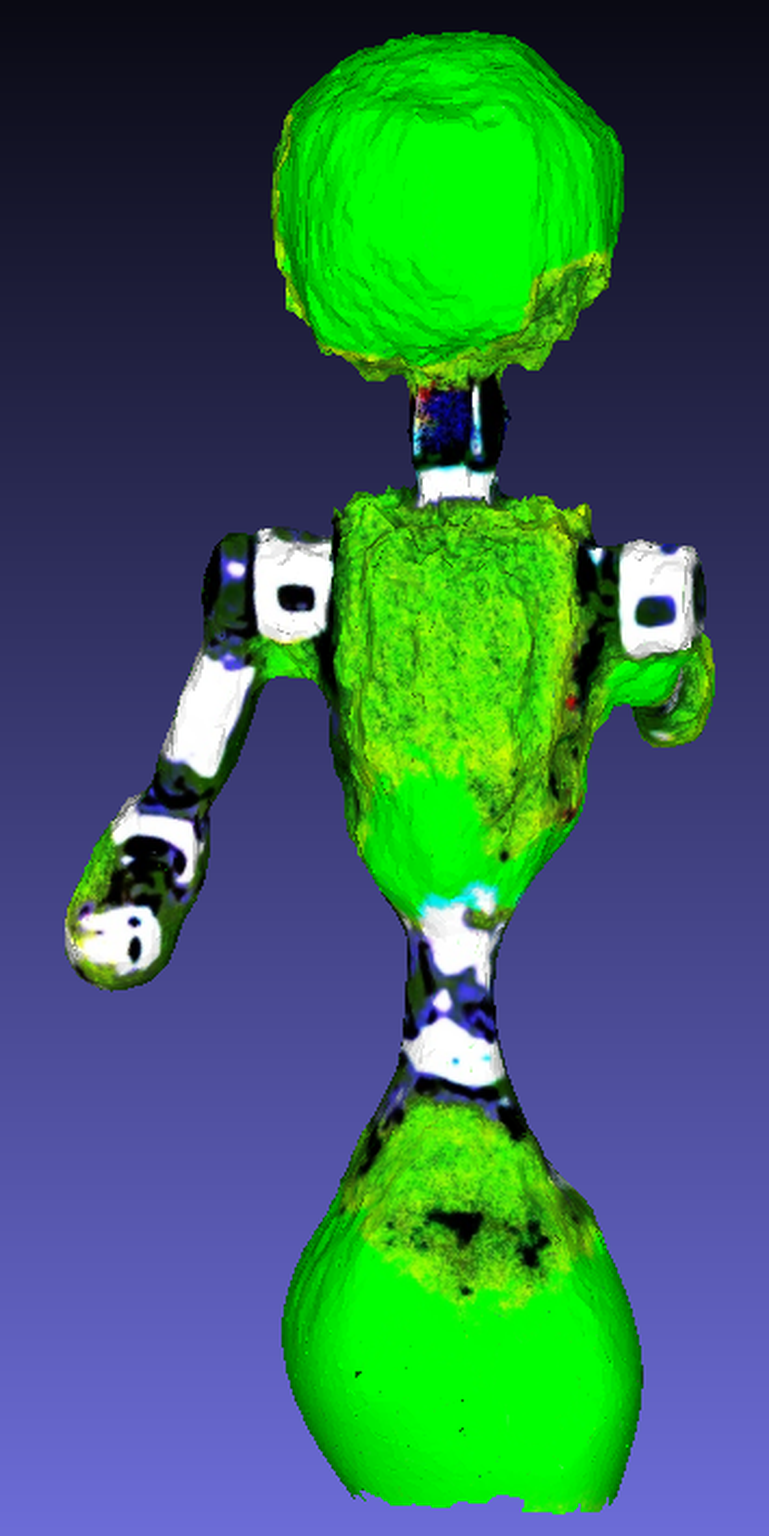
\includegraphics[width=.14\columnwidth]{etc/a robot made out of plants/magic3d/magic3d_plantRobot_model_resized.png}
      \caption{Further results from Magic3D\@: The left image shows the developed albedo texture, while the right image shows the finished 3D mesh model opened in Meshlab}~\label{fig:texturesMagic3D}
\end{figure}
